\newpage
\section{Synthèse de cours du traitement du signal}

\subsection{Reminder on Nyquist-Shannon Theorem}

\paragraph{Theorem :}
A continuous-time signal of finite bandwidth, that has been
sampled, can be perfectly reconstructed from a finite sequence of
samples if the sampling rate exceeds 2F samples per seconds, F being
the highest frequency of the original signal.

\paragraph{}
There are two cases to consider here : 

If the highest frequency of the signal is known and equal to \(f\), we need a sampling frequency superior to \(2f\) to describe it correctly. The frequency \(2f\) is called the \textbf{Nyquist rate}.

Whereas, if only the sampling frequency is known as \(f_S\), it means that the highest frequency of the have to be inferior to \(f_S/2\). The frequency \(f_S / 2\) is called the \textbf{Nyquist frequency} noted here \(f_N\). 

\paragraph{}
If those conditions are not satisfied, aliasing phenomenon can be observed. It means that is the highest frequency of the signal is noted \(f_1\) and \(f_1 > f_N\), the frequency observed is \(f = f_S - f_1\).

\paragraph{}
To avoid it, there are two main possibilities, the first one that can be the most intuitive which is to increase the sampling frequency. Nevertheless, it also possible to use an anti-aliasing filter. It is basically a high-pass filter so it can implies to lose some frequencies in the signal but at least, it is a good tool to be certain that there are no false frequencies measured.


\subsection{Discrete Fourier Transform}

\paragraph{}
The Discrete Fourier Transform (or DFT) is a good way to approach the real value of Fourier Transform by a numerical way, if we consider \(x_j\) \(1 \leq j \leq N\) all the samples of signal separed by a duration \(\Delta t = \frac{1}{f_S}\) and \(X_k\) coefficients referred to the signal spectrum, they verify the relations : 

\begin{gather}
    X_k = \sum_{j=0}^{N-1} x_j e^{2i\pi \frac{j k}{N}} ~~~~~~k=0,\dots,N-1 \\
    x_j = \frac{1}{N}\sum_{k=0}^{N-1} X_k e^{2i\pi \frac{j k}{N}} ~~~~~~ j=0,\dots, N-1
\end{gather}

\subsubsection{Units}

\begin{figure}[h]
    \begin{minipage}{0.5\textwidth}
        Spectral resolution :
    \begin{equation*}
    \Delta f = \frac{f_S}{N}
    \end{equation*}

    Frequency range :
    \begin{equation*}
        f=\left[- \frac{N}{2} +1 ; \frac{N}{2} \right]
    \end{equation*}
    \end{minipage}
    \begin{minipage}{0.5\textwidth}
    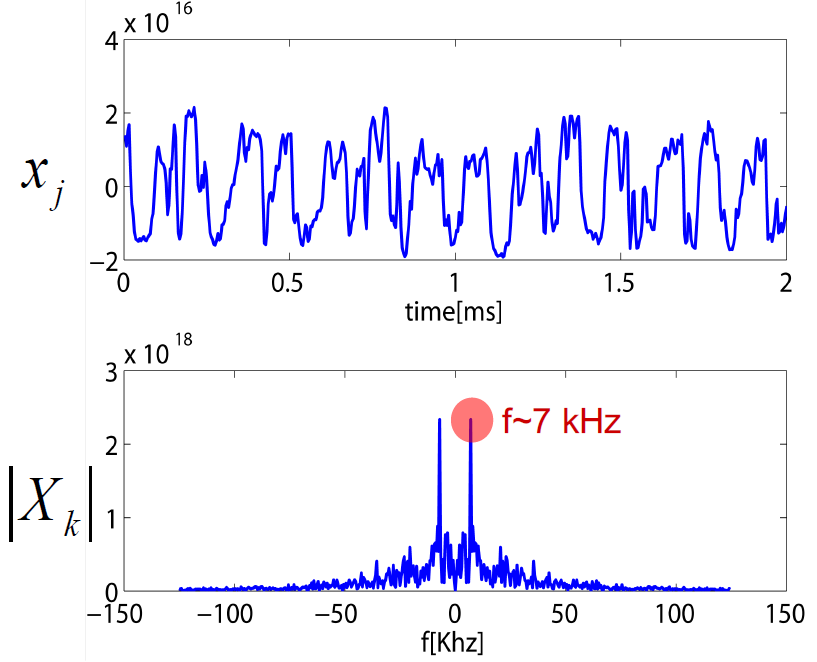
\includegraphics[scale=0.4]{Figures Cours Traitement du Signal/Units of DFT.png}
    \caption{A signal and its DFT}
    \label{fig:DFT example}
    \end{minipage}
\end{figure}

\newpage
\subsubsection{Time-frequency representation : the spectrogram}

One thing that we can notice with the representation of figure \ref{fig:DFT example} is that when DFT (or a classical Fourier Transform) is applied to a signal, we totally lose the information of time. To keep both informations (frequency and time), we use a matrix that is called a spectrogram which allows to represent both. 

\begin{figure}[h]
\begin{minipage}{0.4\textwidth}
    Coefficients of corresponding matrix are are given by : 

    \begin{equation*}
        S_{n,k}=\Delta t \sum_{j=(n-1)M} ^{nM} x_j e^{+2\pi i \frac{j k}{M}}
    \end{equation*}
    With \(1\leq M \leq N\)

    \paragraph{}
    It is a \(N \times (N/M)\) matrix 
\end{minipage}
\begin{minipage}{0.6\textwidth}
\centering
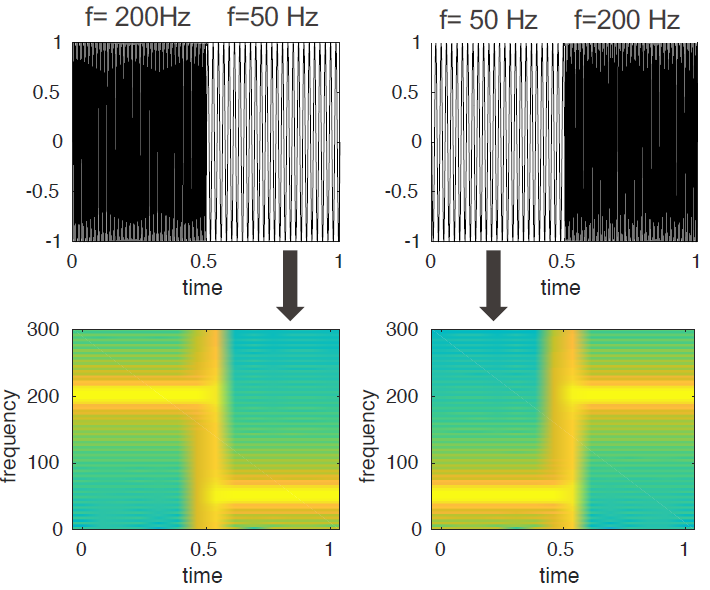
\includegraphics[scale=0.5]{Figures Cours Traitement du Signal/Exemples spectrogrames.png}
\caption{Example of a simple spectrogram}
\label{fig:spectrogram_example}
    
\end{minipage}
\end{figure}

\subsection{Energy of a discret-time signal}

\subsubsection{Total power of a discrete-time signal}

\begin{equation}
    P = \sum_{n=-\infty} ^{+\infty} \mid x[n] \mid ^2
\end{equation}

\paragraph{}
This definition of energy is consistent with the idea that if \(x[n]\) represent a time-varying voltage, the sum is the total energy throughout a 1 Ohm resistance. Indeed, we can find that this sum dimensionnaly equal to a power :

\begin{gather*}
    [U]=M.L^2.T^{-3}.I^{-1} ~~ [R] = M.L^2.T{-3}.I^{-2} \\
    \Rightarrow \left[\frac{U^2}{R}\right] = \frac{M^2. L^4 .T^{-6}.I^{-2}}{M.L^2.T^{-3}.I^{-2}} = M.L^2.T^{-3}=[P]
\end{gather*}

\paragraph{}
Thus, the energy of the signal is equal to : 

\begin{gather}
    E = \Delta t \sum_{n=0} ^{N-1} \mid x[n] \mid ^2
\end{gather}

\paragraph{Energy conservation : } Which comes from Parseval Identity

\begin{equation}
    P=\frac{1}{N} \sum_{n=0} ^{N-1} \mid x[n] \mid ^2 = \frac{1}{N^2} \sum _{j=0} ^{N-1} \mid X[j] \mid ^2
\end{equation}

\subsubsection{Power Spectral density (or PSD) of a discrete-time signal}

The PSD is defined  for zero and positive frequencies : 

\begin{gather*}
    P(0) = \frac{1}{N^2}\mid X_0 \mid ^2 ~~ P(f_n) = \frac{1}{N^2}\left[\mid X_n\mid ^2 + \mid X_{N-n}\mid ^2 \right] ~~~~n= ,\dots, \frac{N}{2}-1 \\
    P(f_N) = \frac{1}{N^2} \left[\mid X_{N/2} \mid ^2 \right]
\end{gather*} 

It is also important to notice that PSD makes no sense outside of the interval \([-f_N ; f_N]\). 

\subsection{Cross-Correlation}

\subsubsection{Idea}

We may say that two signals are correlated if they “follow” each other, or, in
other terms, if we can predict the second signal knowing the first or vice versa. 

\subsubsection{Definition}

Cross-Correlation allows to measure similarity between two signals \(y_1\) and \(y_2\). This can be made thanks to the cross-correlation function : 

\begin{equation}\label{correlation function}
    R_{y_1, y_2} (\tau) = \frac{\sum_{i=0}^{N-\tau - 1} (y_{1,i}- \overline{y_1})(y_{2,i+\tau}-\overline{y_2})}{\sigma_1 \sigma_2}
\end{equation}

\begin{figure}[h]
    \begin{minipage}{0.5\textwidth} 
        \paragraph{}
        This functions gives us informations on the "direction" of fluctuations propagation. Knowing the distance between mesurement points on the spectrogram, this function can give an estimate of the propagation velocity of fluctuations. 
        
        \paragraph{}
        It is also important to notice that the maximum of function is usually not reached at \(t=0\). 
    \end{minipage}
    \begin{minipage}{0.5\textwidth}
        \centering
        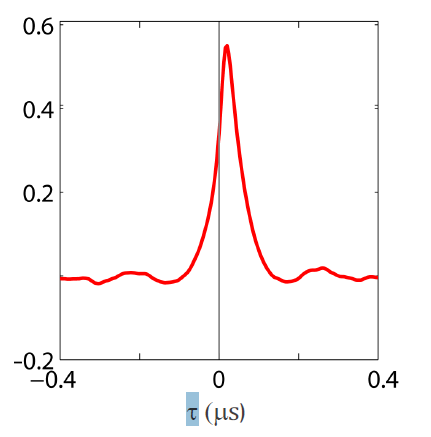
\includegraphics[scale=0.65]{Figures Cours Traitement du Signal/Cross-correlation function.png}
        \caption{Example of cross-correlation function}
        \label{fig:example_cross-correlation_function}
    \end{minipage}
\end{figure}

Compléter la suite après avoir compris.  
\newpage

\subsubsection{Auto-correlation}

If we consider \(y_2 = y_1 = y\), the cross-correlation (\ref{correlation function}) becomes the auto-correlation function :

\begin{equation}
    R_{xx}(\tau) = \frac{\sum_{i=0}^{N-\tau-1}(y_i - \overline{y})(y_{i+\tau}-\overline{y})}{\sigma_y ^2}
\end{equation}


\subsection{Statistical methods}

\subsubsection{Random variables and Probability Distribution Function (or PDF)}

First, we introduce the Cumulative Distribution Function which measures the probability that the variable \(x\) takes a smaller value than \(\alpha\) a number : 

\begin{gather*}
    F_x(\alpha) = P[x \leq \alpha]
\end{gather*}

The probability Density Function is related to CTDF as : 
\begin{equation*}
    f_x (\alpha) = \frac{\textrm{d}F_x (\alpha)}{\textrm{d}\alpha} ~~~~ F_x (\alpha) = \int_{-\infty}^{\alpha}f_x(x) \textrm{d}x
\end{equation*}

\newpage
\subsubsection{How to compute PDF in practice with discrete data ?}

\begin{figure}[h]
\begin{minipage}{0.5\textwidth}
   \paragraph{}
    It consists in dividing signal into bins and to count the number of samples in each bin which takes a value inferio or equal to \(\alpha\). The ideal number of bins is \(\sqrt{N}\), it is the one which provides best statistics. 

\paragraph{}
As a Probability Distribution Function, the function have also to be normalised : 

\begin{equation*}
    \int_{-\infty} ^{+\infty} f_x (x) \textrm{d}x = 1 
\end{equation*}
\end{minipage}
\begin{minipage}{0.5\textwidth}
    \centering
    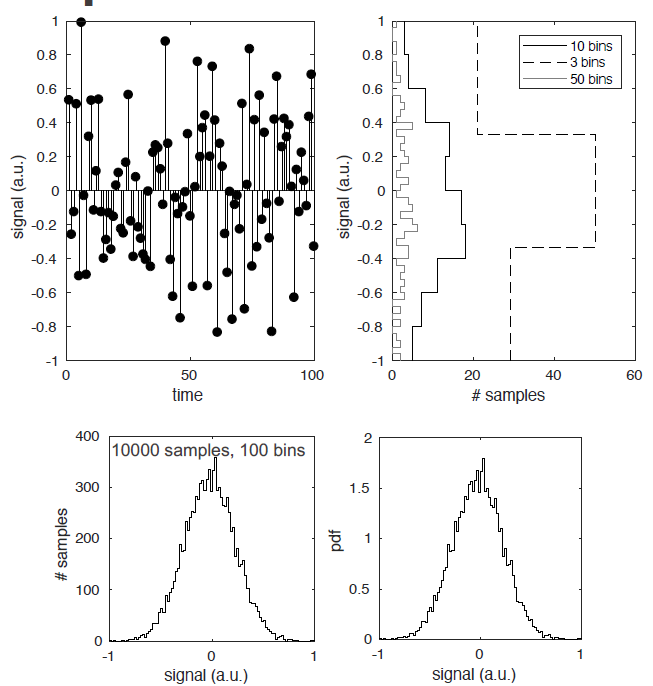
\includegraphics[scale=0.4]{Figures Cours Traitement du Signal/PDF in practice from discrete data.png}
    \caption{Construction of Probability Distribution Function}
    \label{fig:PDF}
\end{minipage}
\end{figure}

\subsubsection{Moments of the PDF}

\paragraph{Mean :}
\begin{equation}
    \overline{x} = \frac{1}{N} \sum_{j=0}^{N-1} x_j
\end{equation}

\paragraph{Variance :}

\begin{equation}
    \sigma^2 = \frac{1}{N-1} \sum_{j=0} ^{N-1} (x_j - \overline{x})^2
\end{equation}

\paragraph{Skewness :}
Third order moment, it "measures" the asymetry of the data around the samples mean. The skewness of the normal distribution (or any perfectly symetric distribution) is zero. 

\begin{equation}
    sk= \frac{1}{N} \sum_{j=0} ^{N-1} \left[\frac{x_j-\overline{x}}{\sigma}\right]^3
\end{equation}

\paragraph{Kurtosis (or Flatness) :}
Fourth order moment, it "measures" the peaking of the PDF with respect to the normal distribution. Kurtosis is a measure of how outlier-prone a distribution is. The kurtosis of normal distribution is 0. 

\begin{equation}
    kur = \frac{1}{N}\sum_{j=0}^{N-1}\left[\frac{x_j - \overline{x}}{\sigma}\right]^4-3
\end{equation}

\paragraph{Interest :}
The idea is to compare a data set to a known distribution or to compare two or more data sets distributions in order to get informations on physical process behind the data. 

\paragraph{}
The most commonly accepted test for comparing different binned PDFs is the Chi-squared test. 

\begin{equation}
    \chi^2 = \frac{1}{N=1}\sum_{j=0}^{N-1} (x_{exp} - x_{th})^2
\end{equation}

\subsubsection{PLASMAS}

\subsubsection{How to extract coherent structures : conditionnal averaging}

\paragraph{}
A signal can be decomposed with a time-dependent part and a fluctuating part : \(y(x,t) = \overline{y}(x) + \Tilde{y}(x,t)\)

\paragraph{}
The fluctuating part can be decomposed with a \textbf{coherent} part and a \textbf{random} one : \(y(x,t) = \overline{y} (x) + \tilde{y}_{coh} (x,t) + \tilde{y}_{rand}(x,t)\). An ensemble average over a lot of independent realization will remove the random part :

\begin{gather*}
    \langle \tilde{y}(x,t) \rangle = \langle \tilde{y}_{coh}(x,t) + \tilde{y}_{rand}(x,t) \rangle = \langle \tilde{y}_{coh}(x,t) \rangle + \langle \tilde{y}_{rand}(x,t) \rangle = \langle \tilde{y}_{coh}(x,t) \rangle 
\end{gather*}

\subsubsection{How to build an ensemble of independent realizations ?}

\begin{figure}[h]
    \begin{minipage}{0.5\textwidth}
        \paragraph{}
        The first step is to select a criterion : \(y_0 < y < y_0 + \Delta y_0\). Then, we have to select a time window : \(t_i - \Delta t < t < t_i + \Delta t \) where \(\Delta t\) is of the order of autocorellation time. 

        \paragraph{}
        The ensemble of independent realizations is obtained when the same time windows are identified in other signals. 
    \end{minipage}
    \begin{minipage}{0.5\textwidth}
    \centering
    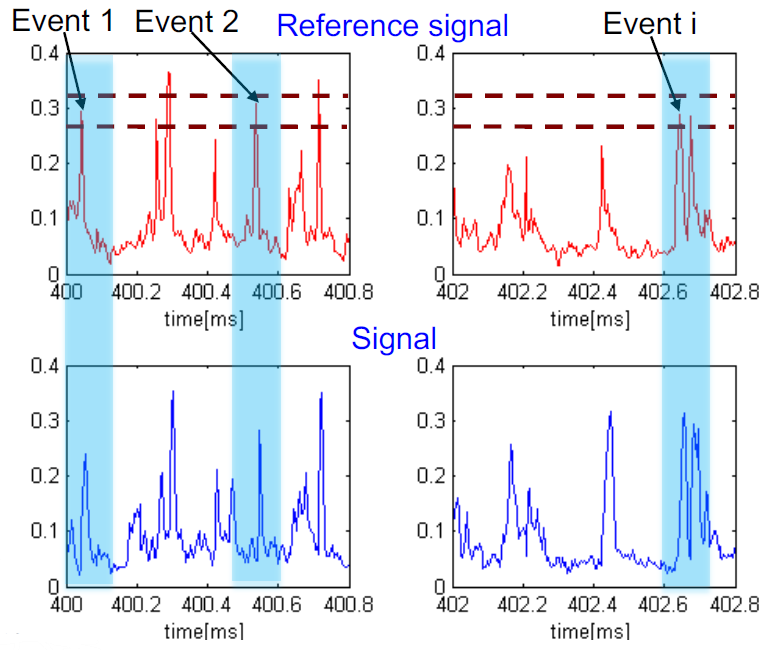
\includegraphics[scale=0.4]{Figures Cours Traitement du Signal/How to build independent realizations.png}
    \caption{}
    \label{fig:how to build an ensemble of independent realizations}
    \end{minipage}
\end{figure}

\subsubsection{Conditionnal averaging}

We Consider two signals : a reference signal and a "useful" signal. The figures \ref{fig:conditionnal averaging} is get when identified time windows are put together for the reference signal and the "useful" signal. 

\begin{figure}[h]
    \begin{minipage}{0.5\textwidth}
        \centering
        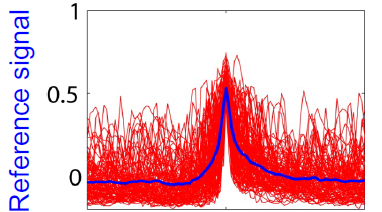
\includegraphics[scale=0.8]{Figures Cours Traitement du Signal/Reference signal 1.png}
    \end{minipage}
    \begin{minipage}{0.5\textwidth}
        \centering
        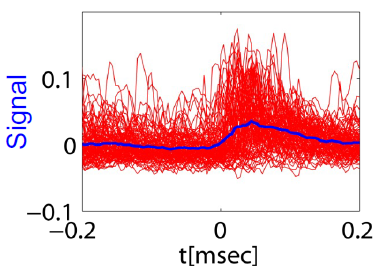
\includegraphics[scale=0.8]{Figures Cours Traitement du Signal/Useful Signal - 2.png}
    \end{minipage}
    \caption{}
    \label{fig:conditionnal averaging}
\end{figure}

\paragraph{}
The maxima in the average reference signal and in the average "useful" signal are not reached at the same time. 

\newpage
\subsubsection{Conditional averaging allows reconstructing 2D/3D
dynamics}

\begin{figure}[h]
    \begin{minipage}{0.5\textwidth}
        \paragraph{}
        The red probe is the reference probe, fixed and detecting an event. The blue probe ("useful" probe) is moved between two shots over the green area to sample 2D dynamics of a coherent event. It can measure a different quantity from the reference probe.

        \paragraph{IMPORTANT :} 
        The signals have to be stationary to shot-to-shot reproductibility. 
    \end{minipage}
    \begin{minipage}{0.5\textwidth}
        \centering
        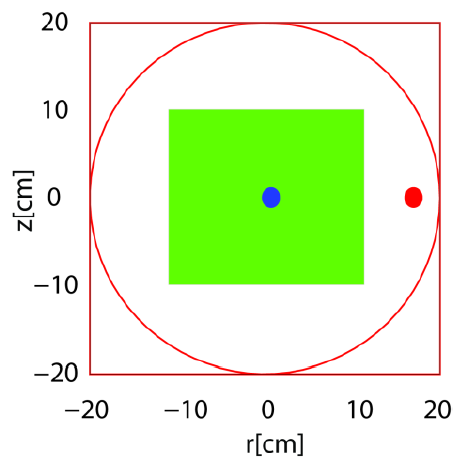
\includegraphics[scale=0.4]{Figures Cours Traitement du Signal/2D 3D.png}
        \caption{Representation of both probes}
        \label{fig:2D/3D synamics}
    \end{minipage}
    
\end{figure}